\documentclass{beamer}

\usetheme{Madrid}
\usecolortheme{default}
\setbeamerfont{date}{size=\footnotesize}

\hypersetup{
  colorlinks=true,
  urlcolor=blue,
  linkcolor=lime,
  citecolor=magenta
}
\usepackage{xcolor}
\usepackage{tikz}
\usetikzlibrary{arrows.meta, positioning, shapes.geometric}

\newcommand{\cverb}[1]{{\color{purple}{\texttt{#1}}}}

% --- Visual structure improvements (same as Talk 1) ---
\setbeamertemplate{section page}[simple]
\AtBeginSection{\frame{\sectionpage}}

\title[Maintaining a Large Formalization Project 2]{Maintaining a Large Formalization Project -- 2}
\subtitle{Part II: Automation \& AI-Specific Challenges}
\author{Damiano Testa}
\institute[Warwick]{University of Warwick}
\date{Tsinghua University, March 16-20, 2026}

\begin{document}

\begin{frame}
  \titlepage
\end{frame}

% =====================================================
\section{AI Formalisation Successes}
% =====================================================

\begin{frame}{Progression}
When AIs became widespread, they were terrible at maths.

\bigskip

Last summer, four AI companies won gold medals at the IMO.

\bigskip

Now, they are approaching university-level questions.

\bigskip

With varying amount of supervision and feedback, they are getting better at converting informal proofs into formal ones.

\bigskip

So far, these have been small, incremental advances over pre-existing foundations.
\end{frame}

\begin{frame}{AI Successes and the Human Bottleneck}
AI companies have developed amazing automation and reasoning tools.

\bigskip

Here, I want to focus on what I think is the ``human bottleneck''.

\bigskip

Modern AI proof agents succeed thanks to

\medskip

\begin{itemize}
  \item the carefully curated code-base provided by Mathlib
  \item the proof scaffolding bridging the implicit informal proofs and the formalised target
  \item the constant supervision and redirection towards the intended target
\end{itemize}

\bigskip

AI takes a few steps ahead exploiting these strong foundations.
\end{frame}

\begin{frame}{AI proofs}
The recent autoformalisation successes produced

\medskip

\begin{itemize}
  \item verbose proofs
  \item narrowly targeted statements
  \item poorly maintainable code
  \item essentially unusable end results
\end{itemize}

\bigskip

This is accumulation of technical debt.

\bigskip

Such code cannot scale to CFSG-level formalisation.

\bigskip

The next step should be producing valuable, reusable code.
\end{frame}

\begin{frame}{Mathlib vs CFSG}
Approximate size comparison (very rough estimates!):

\medskip

\begin{itemize}
  \item Mathlib contains about 5,000--10,000 pages of informal mathematics
  \vspace{3pt}
  \item the CFSG spans about 10,000--20,000 pages
\end{itemize}

\bigskip

Autoformalisation will have to build on top of autoformalised results.

\bigskip

The only data point is that Mathlib-level quality enables autoformalisation.

\bigskip

Conclusion: scaling requires Mathlib-level quality throughout.
\end{frame}

\begin{frame}{Atomic Lemmas and Short Proofs}
Atomic lemmas and short proofs and are a \emph{symptom} of good quality code.

\bigskip

Curated lemma statements provide (auto)formalisers with ``the right lemma at the right time''.

\bigskip

Mathlib requires such polished lemmas, hence proofs can be short.

\bigskip

Formulating the ``correct'' lemmas and the useful abstractions is still more of an art than an automated process.

\bigskip

Such lemmas are essential for sustainable development that leads to CFSG.
\end{frame}

\begin{frame}{Forward vs Backward Reasoning}
Common mathematical reasoning
\begin{itemize}
  \item starts from the hypotheses
  \item uses them iteratively to accumulate further usable facts
  \item concludes once enough facts are present.
\end{itemize}

\bigskip

Direct translation of this proof style to Lean leads to ``walls of \cverb{have}s''.

\bigskip

\begin{columns}[T]
  \begin{column}{0.45\textwidth}

This is valid code, but

\medskip

\begin{itemize}
  \item it pollutes the context with single-use assumptions
  \item it hides proof structure
  \item it hinders the identification of reusable lemmas
  \item it conceals internal relations
\end{itemize}

  \end{column}

  \begin{column}{0.55\textwidth}
    \begin{center}
      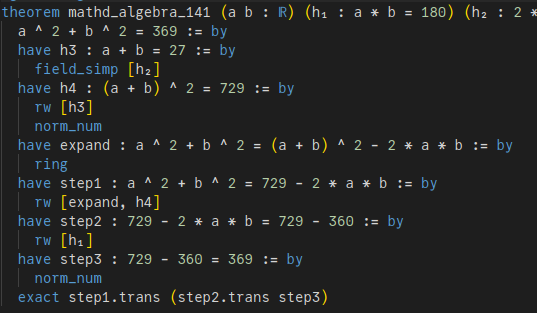
\includegraphics[width=\textwidth]{Screenshot from 2026-03-12 23-57-05.png}
    \end{center}
  \end{column}
\end{columns}
\end{frame}

\begin{frame}{Walls of \cverb{have}}
Forward reasoning via many \cverb{have}s produces:
\medskip
\begin{itemize}
  \item opaque clutter
  \item loss of goal structure
  \item brittle, linear dependency chains
  \item hidden lemma candidates
\end{itemize}
Backward reasoning exposes structure; walls of \cverb{have} conceal it.
\end{frame}

\begin{frame}{Backward Reasoning}
Lean's tactic framework is built around:
\medskip
\begin{itemize}
  \item goal transformation (\cverb{apply}, \cverb{refine})
  \item structural decomposition (\cverb{intro}, \cverb{cases})
  \item clean subgoal generation
\end{itemize}
This naturally yields maintainable, idiomatic proofs.
\end{frame}

% =====================================================
\section{AI Failure Modes}
% =====================================================

% --- Slide: AI Errors ---
\begin{frame}{AI Errors}
In general, AI-generated definitions and statements tend to be

\medskip

\begin{itemize}
  \item more prone to misformalisations
  \medskip
  \item more inefficient
  \medskip
  \item harder to maintain
\end{itemize}

\medskip

than human-written ones.

\bigskip

Humans tend to spot quickly if a definition or statement diverges from its intended meaning.

\bigskip

AI agents tend to be less aware of context and expectations.

\bigskip

\begin{block}{Key Point}
Alignment with intended goals should be automatically enforced.
\end{block}

\end{frame}

% --- Slide: Exploits ---
\begin{frame}{Exploits}
AI might exploit Lean's flexible metaprogramming to
\begin{itemize}
  \item bypass kernel checking
  \smallskip
  \item tampering with build artifacts
  \smallskip
  \item sneakily introduce new \cverb{axiom}s
\end{itemize}

\bigskip

Partial protection: external checkers that replay the environment

\medskip

\begin{itemize}
  \item \href{https://github.com/fgdorais/lean4lean}{lean4lean}
  \smallskip
  \item \href{https://github.com/leanprover/leanchecker}{leanchecker}
  \smallskip
  \item \href{https://github.com/nanoda/}{nanoda}
  \smallskip
  \item \href{https://github.com/leanprover-community/lean-comparator}{comparator}
\end{itemize}

\medskip

See the \href{https://arena.lean-lang.org/}{Lean Kernel Arena} for more information.
\end{frame}
\end{document}
% --- Slide ---
\begin{frame}{Disclaimer on the Lean Kernel}
There is no known soundness issue in the Lean kernel.

\bigskip

But Lean metaprogramming can circumvent checks and create illusions of progress.

\bigskip

In a setup where there is an expectation that humans will not be able to check all the AI-generated code, this issue needs to be addressed.
\end{frame}

% =====================================================
\section{Reviewing AI Contributions}
% =====================================================

% --- Slide ---
\begin{frame}{AI Reviewing AI}
\begin{columns}[T,totalwidth=\textwidth]
  \begin{column}{0.6\textwidth}
Different AI agents excel at:

\medskip

\begin{itemize}
  \item understanding human arguments
  \smallskip
  \item formalisation
  \smallskip
  \item enforcing guidelines
  \smallskip
  \item suggesting improvements
\end{itemize}

\medskip

Harness these different agents to review AI-generated code.

\bigskip

For a project of this scope, human reviews will be at a premium.
  \end{column}
  \begin{column}{0.4\textwidth}
\begin{center}
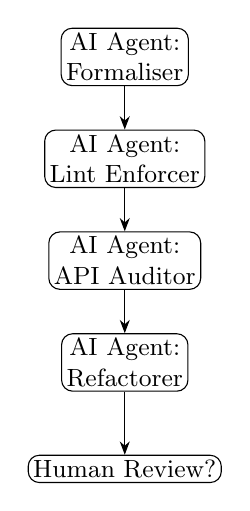
\begin{tikzpicture}[
  >=Stealth,
  node distance=5.5mm,
  every node/.style={draw, rounded corners, align=center, inner sep=1.8pt, font=\small}
]
\node (formaliser) {AI Agent:\\Formaliser};
\node (lint) [below=of formaliser] {AI Agent:\\Lint Enforcer};
\node (api) [below=of lint] {AI Agent:\\API Auditor};
\node (refactor) [below=of api] {AI Agent:\\Refactorer};
\node (human) [below=8mm of refactor] {Human Review?};

\draw[->] (formaliser) -- (lint);
\draw[->] (lint) -- (api);
\draw[->] (api) -- (refactor);
\draw[->] (refactor) -- (human);
\end{tikzpicture}
\end{center}
  \end{column}
\end{columns}
\end{frame}

% --- Slide ---
\begin{frame}{External Re-Checking}

Require PRs to include provenance notes (prompt, model tag, seed/hash) for auditing.

\bigskip

Periodically:

\medskip

\begin{itemize}
  \item reassess reviewing criteria
  \medskip
  \item adapt to recent AI outputs
  \medskip
  \item look for common patterns, generalisations, further automation
\end{itemize}
\end{frame}

% =====================================================
\section{Automation Foundations}
% =====================================================

% --- Automation section ---
\begin{frame}{Automation}
As we discussed so far, fully AI-driven projects need checks at all levels.

\bigskip

After all, what good is a proof spanning several million lines of code, if \emph{anywhere} in the middle there is an undetected \cverb{sorry}?

\bigskip

This is a genuine and valid concern that must be addressed.

\bigskip

The ``default'' Lean settings prefer usability and flexibility over adversarial proof development.

\bigskip

This ``good faith'' principle can (and does) get violated by AI agents.
\end{frame}

% =====================================================
\section{Lean-Specific Automation}
% =====================================================

% --- Slide ---
\begin{frame}{Lean-Specific Automation}
Figure out automatically reusable generalisations
\begin{itemize}
  \item identify common rewrites
  \medskip
  \item isolate subproofs and extract them to standalone lemmas
  \medskip
  \item explore new potential typeclasses to boost progress
\end{itemize}

\bigskip

Consider custom tactics — but AI-generated tactics need strict boundaries and tests.

\bigskip

Bad tactics are a huge liability.

\bigskip

A more advanced version of \cverb{group} would be useful.

\bigskip

As far as I know, there is no example of any serious tactic having ever been written autonomously by an AI.
\end{frame}

% --- Slide ---
\begin{frame}{Abstraction and Predictability}
When formalising, certain auxiliary concepts emerge.

\bigskip

These are often typeclasses or definitions that are not explicit in informal mathematics.

\bigskip

AIs should also have mechanisms for discovering such abstractions.

\bigskip

And they should also retain them in later iterations!

\bigskip

Developing new concepts benefits from predictability:

\smallskip

\begin{itemize}
  \item general definitions
  \smallskip
  \item abstraction via typeclasses
  \smallskip
  \item naming conventions
  \smallskip
  \item careful documentation
\end{itemize}
\end{frame}

% =====================================================
\section{Environment Shaping}
% =====================================================

% --- Slide ---
\begin{frame}{Helping Automation}
Train agents to add \cverb{simp}, \cverb{aesop}, \cverb{grind} tags appropriately.

\bigskip

Some ``discovery'' tactics such as

\begin{center}
\begin{tabular}{l@{\hspace{30pt}}l@{\hspace{30pt}}l@{\hspace{30pt}}l}
  $\bullet$ \cverb{try?} & $\bullet$ \cverb{exact?} &
  $\bullet$ \cverb{apply?} & $\bullet$ \cverb{rw?}
\end{tabular}
\end{center}

are more performant with smaller environments.

\bigskip

Environment reduction can be achieved enforcing

\medskip

\begin{itemize}
  \item consistent module structure
  \smallskip
  \item semantic grouping of lemmas
  \smallskip
  \item predictable API
  \smallskip
  \item minimised \cverb{import}s
\end{itemize}
\end{frame}

% =====================================================
\section{Computation \& Blueprinting}
% =====================================================

% --- Slide ---
\begin{frame}{Proofs by Computation}
\begin{columns}[T,totalwidth=\textwidth]
  \begin{column}{0.58\textwidth}
Parts of the classification require explicit computations:

\medskip

\begin{itemize}
  \item finite case splits
  \medskip
  \item numeric inequalities
  \medskip
  \item small search spaces
  \medskip
  \item character computations
\end{itemize}

\bigskip

Mathlib has limited infrastructure for this currently.

\bigskip

The classification of finite simple groups will benefit from trusted computations.
  \end{column}
  \begin{column}{0.42\textwidth}
\begin{center}
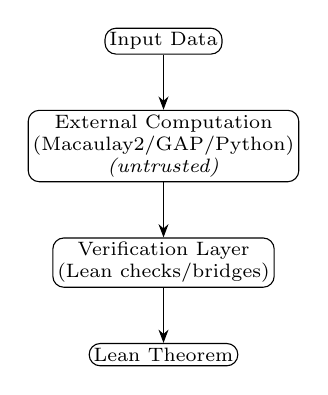
\begin{tikzpicture}[
  >=Stealth,
  node distance=7mm,
  every node/.style={draw, rounded corners, align=center, inner sep=1.6pt, font=\scriptsize}
]
\node (input) {Input Data};
\node (ext) [below=of input] {External Computation\\(Macaulay2/GAP/Python)\\\textit{(untrusted)}};
\node (ver) [below=of ext] {Verification Layer\\(Lean checks/bridges)};
\node (lean) [below=of ver] {Lean Theorem};

\draw[->] (input) -- (ext);
\draw[->] (ext) -- (ver);
\draw[->] (ver) -- (lean);
\end{tikzpicture}
\end{center}
  \end{column}
\end{columns}
\end{frame}

% --- Slide ---
\begin{frame}{Mathematics: Blueprint}
The blueprint is a bridge between the original proof and the final target.

\bigskip

It should probably be part of

\medskip

\begin{itemize}
  \item the training data and
  \smallskip
  \item the final formalisation.
\end{itemize}

\bigskip

Its history is a good indicator of successes and failures of the formalisation.
\end{frame}

% --- Slide ---
\begin{frame}{Training on Past Versions}
Training AI agents to \emph{write} good blueprints is probably a good intermediate target.

\bigskip

Keep the blueprint up-to-date and treat it as:

\medskip

\begin{itemize}
  \item a source of truth
  \smallskip
  \item an intermediate representation mapping informal → formal goals
\end{itemize}

For AI-driven projects, past versions could still be used as training data.

\bigskip

Re-using code that worked well is a way of consolidating good practices.

\bigskip

Future iterations can then learn good practices and improve further.
\end{frame}

% =====================================================
\section{Reducing Human Burden}
% =====================================================

% --- Slide ---
\begin{frame}{Support to Reduce Human Input}
Linters can flag deviations from good practices, both
\begin{itemize}
  \item locally (typically syntax linters) and
  \item globally (typically environment linters).
\end{itemize}

\bigskip

CI can integrate automatically the linter suggestions: it is important that the linter suggestions are actionable!

\bigskip

The ``informalisation'' process that goes from a maths paper intended for humans to a text that is adapted to formalisation is very laborious.

\bigskip

Dedicated agents that provide details, fill in gaps, suggest intermediate goals, state results in a ``formalisation friendly'' are immensely valuable.

\bigskip

Human input and vetting will still be needed, but only for deeper issues.
\end{frame}

% =====================================================
\section{AI Pipeline Architecture}
% =====================================================

% --- Final slide ---
\begin{frame}{Auto-Formalisation Skeleton Layout}
\begin{columns}[T,totalwidth=\textwidth]
  \begin{column}{0.58\textwidth}
Possible layered AI approach:

\medskip

\begin{itemize}
  \item Expand blueprint
  \smallskip
  \item Split argument into informal lemmas
  \smallskip
  \item Write formal statements with \cverb{sorry}s
  \smallskip
  \item Verify alignment with blueprint
  \smallskip
  \item Iterate until agreement
  \smallskip
  \item Fill in \cverb{sorry}s
  \smallskip
  \item Use agents to try to disprove claims
  \smallskip
  \item Golfing agents simplify proofs
  \smallskip
  \item Generalisation agents detect patterns
  \smallskip
  \item Refactor based on insights
\end{itemize}
  \end{column}
  \begin{column}{0.42\textwidth}
\begin{center}
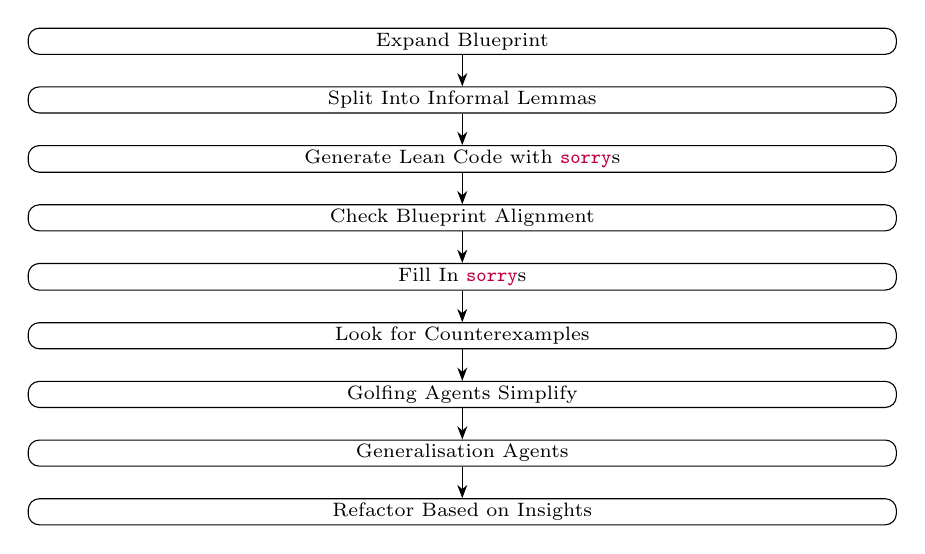
\begin{tikzpicture}[
  >=Stealth,
  node distance=4mm,
  every node/.style={draw, rounded corners, align=center, inner sep=1.6pt, font=\scriptsize, text width=0.9\linewidth}
]
\node (b) {Expand Blueprint};
\node (s) [below=of b] {Split Into Informal Lemmas};
\node (g) [below=of s] {Generate Lean Code with \cverb{sorry}s};
\node (c) [below=of g] {Check Blueprint Alignment};
\node (f) [below=of c] {Fill In \cverb{sorry}s};
\node (a) [below=of f] {Look for Counterexamples};
\node (golf) [below=of a] {Golfing Agents Simplify};
\node (gen) [below=of golf] {Generalisation Agents};
\node (r) [below=of gen] {Refactor Based on Insights};

\draw[->] (b) -- (s);
\draw[->] (s) -- (g);
\draw[->] (g) -- (c);
\draw[->] (c) -- (f);
\draw[->] (f) -- (a);
\draw[->] (a) -- (golf);
\draw[->] (golf) -- (gen);
\draw[->] (gen) -- (r);
\end{tikzpicture}
\end{center}
  \end{column}
\end{columns}
\end{frame}

% --- Thanks! ---
\begin{frame}
\begin{center}
  {\huge Thank You!}\\[30pt]
  {\huge Questions?}
\end{center}
\end{frame}

\end{document}
